%&pdflatex
\documentclass[12pt]{article}
\usepackage[margin=1.0in]{geometry}

\usepackage{g-util}
\usepackage{amsfonts, amsmath, amssymb}
\usepackage{graphicx, float}

\graphicspath{ {../data/} }
%\usepackage[xetex]{xcolor}

% \theoremstyle{plain}
  \newtheorem{prop}{Proposición}
  \newtheorem{lema}{Lema}
% \theoremstyle{remark}
  \newtheorem{obs}{Observación}
% \theoremstyle{definition}
  \newtheorem{defi}{Definición}

\setcounter{MaxMatrixCols}{12}
\newcommand{\Gpmatrix}[1]{\ensuremath{\begin{pmatrix} #1 \end{pmatrix}}}
\newcommand{\Gbmatrix}[1]{\ensuremath{\begin{bmatrix} #1 \end{bmatrix}}}
\newcommand{\sub}[3]{\ensuremath{#1_{#2,#3}}}
\newcommand{\supra}[2]{\ensuremath{#1^#2}}

\title{Métodos Numéricos}
\author{F. Galileo Cappella Lewi}
\date{1c2022}

\renewcommand{\figurename}{Fig.}
\renewcommand{\listfigurename}{Figuras}
\renewcommand{\contentsname}{Secciones}

\begin{document}

\maketitle

\section{Introducción}

%TODO: Contar el problema que nos presentaron
En general vamos a estar trabajando con \(m+1\) radios, y \(n\) ángulos.

\section{Formulación del Sistema}
 
\paragraph{} Partimos de la ecuación de Laplace \\
\[
  0 = \frac{\partial^2T(r,\ \theta)}{\partial r^2} + \frac{1}{r} \frac{\partial^2T(r,\ \theta)}{\partial r} + \frac{1}{r^2} \frac{\partial^2T(r,\ \theta)}{\partial\theta^2}
\]
Y la discretizamos \\ %TODO: Pasos y justificación en el medio?
\[
0 = \frac{\sub{t}{j-1}{k} - 2\sub{t}{j}{k} + \sub{t}{j+1}{k}}{(\Delta r)^2} + \frac{\sub{t}{j}{k} - \sub{t}{j-1}{k}}{r \Delta r} + \frac{\sub{t}{j}{k-1} - 2\sub{t}{j}{k} + \sub{t}{j}{k+1}}{r^2 (\Delta \Theta)^2}
\]
Podemos reescribir la ecuación como una combinación lineal de cinco temperaturas \\
\begin{align} %TODO: Más chiquita
0 = \sub{t}{j-1}{k} (\frac{1}{(\Delta r)^{2}} + \frac{-1}{r \Delta r}) + \sub{t}{j}{k} (\frac{-2}{(\Delta r)^2} + \frac{1}{r \Delta r} + \frac{-2}{(r \Delta \Theta)^{2}}) + \sub{t}{j+1}{k} \frac{1}{(\Delta r)^{2}} + \sub{t}{j}{k-1} \frac{1}{(r \Delta \Theta)^{2}} + \sub{t}{j}{k+1} \frac{1}{(r\Delta \Theta)^{2}}
\end{align}
Para simplificar la notación vamos a nombrar cada coeficiente \\ %TODO: Renombrar coeficientes para que tengan más sentido
\(
\tab \alpha_r = \frac{1}{(\Delta r)^{2}} + \frac{-1}{r \Delta r} \\
\tab \beta_r = \frac{-2}{(\Delta r)^2} + \frac{1}{r \Delta r} + \frac{-2}{(r \Delta \Theta)^{2}} \\
\tab \gamma_r = \frac{1}{(\Delta r)^{2}} \\ 
\tab \chi_r = \frac{1}{(r \Delta \Theta)^{2}}
\) \\\\
Resaltamos cuatro formas diferentes de escribir la ecuación \\
\begin{align}
  \alpha \sub{t}{j-1}{k} + \beta \sub{t}{j}{k} + \gamma \sub{t}{j+1}{k} + \chi \sub{t}{j}{k-1} + \chi \sub{t}{j}{k+1} = 0 \\
  \beta \sub{t}{j}{k} + \gamma \sub{t}{j+1}{k} + \chi \sub{t}{j}{k-1} + \chi \sub{t}{j}{k+1} = -\alpha \sub{t}{j-1}{k} \\
  \alpha \sub{t}{j-1}{k} + \beta \sub{t}{j}{k} + \chi \sub{t}{j}{k-1} + \chi \sub{t}{j}{k+1} = -\gamma \sub{t}{j+1}{k} \\
  \beta \sub{t}{j}{k} + \chi \sub{t}{j}{k-1} + \chi \sub{t}{j}{k+1} = -\alpha \sub{t}{j-1}{k} - \gamma \sub{t}{j+1}{k}
\end{align}
\\
\paragraph{} Por lo que podemos armar un sistema de ecuaciones de la forma \(Ax = b\) donde cada fila del sistema se corresponde a una instancia de la ecuación de Laplace discretizada. \\
Pero qué forma tiene cada instancia depende de si la temperatura del radio anterior o la del siguiente también son incógnitas (por lo que tienen su coeficiente en la matriz), o si son datos medidos (por lo que cambian al resultado): \\
\tab El primer y último radios (\(\sub{t}{1}{k}\) y \(\sub{t}{m+1}{k}\)) son datos medidos, por lo que no hace falta estimarlos con una ecuación. \\
\tab Como las temperaturas del radio anterior las conocemos (porque son las temperaturas internas medidas), las primeras \(n\) filas (que se corresponden con el radio \(\sub{t}{2}{k}\)) van a tener la forma de la ecuación (3). \\ %TODO: Hyperlink
\tab Luego, las siguientes \((m-2)n\) filas (que son todos los otros radios excepto el \(\sub{t}{m}{k}\)) tienen tanto al radio anteriro como el siguiente incógnitas, por lo que tienen la forma de la ecuación (2). \\ %TODO: Hyperlink
\tab Y las últimas \(n\) filas (radio \(\sub{t}{m}{k}\)) tienen la forma de la ecuación (4). \\ %TODO: Hyperlink
Entonces nos queda una matriz \(A \in \mathbb{R}^{((m-1)n \times (m-1)n)}\) armada de la forma explicada recién, el vector de incógntias \(x \in \mathbb{R}^{(m-1)n}\) con los radios "estirados" uno arriba del otro, y el vector de resultados \(b \in \mathbb{R}^{(m-1)n}\) que tiene las temperaturas medidas en las primeras y últimas \(n\) filas, y el resto 0's.

\paragraph{} El caso de un sistema con 3 radios es especial, ya que para el radio \(\sub{t}{2}{k}\) (que es el vector de incógnitas completo) conocemos tanto las temperaturas del radio anterior como del siguiente. Sólo en este caso tenemos la ecuación (5).

\subsection{Justificación no-pivoteo} 
\label{sec:justificacion}

%TODO

\subsection{Ejemplos}

\paragraph{3 radios y 4 ángulos:} \ \\

\(
\Gpmatrix{
  \beta & \chi & 0 & \chi \\
  \chi & \beta & \chi & 0 \\
  0 & \chi & \beta & \chi \\
  \chi & 0 & \chi & \beta \\
} \cdot \Gpmatrix{
  \sub{t}{2}{1} \\
  \sub{t}{2}{2} \\
  \sub{t}{2}{3} \\
  \sub{t}{2}{4} \\
} = \Gpmatrix{
  -\alpha\sub{t}{1}{1} - \gamma\sub{t}{3}{1} \\
  -\alpha\sub{t}{1}{2} - \gamma\sub{t}{3}{2} \\
  -\alpha\sub{t}{1}{3} - \gamma\sub{t}{3}{3} \\
  -\alpha\sub{t}{1}{4} - \gamma\sub{t}{3}{4} \\
}
\)

%\paragraph{4 radios y 4 ángulos:} \ \\

%\(
%\Gpmatrix{
  %\beta & \chi & 0 & \chi & -\gamma & 0 & 0 & 0 \\
  %\chi & \beta & \chi & 0 & 0 & -\gamma & 0 & 0 \\
  %0 & \chi & \beta & \chi & 0 & 0 & -\gamma & 0 \\
  %\chi & 0 & \chi & \beta & 0 & 0 & 0 & -\gamma \\
  %-\alpha & 0 & 0 & 0 & \beta & \chi & 0 & \chi \\
  %0 & -\alpha & 0 & 0 & \chi & \beta & \chi & 0 \\
  %0 & 0 & -\alpha & 0 & 0 & \chi & \beta & \chi \\
  %0 & 0 & 0 & -\alpha & \chi & 0 & \chi & \beta \\
%} \cdot \Gpmatrix{
  %\sub{t}{2}{1} \\
  %\sub{t}{2}{2} \\
  %\sub{t}{2}{3} \\
  %\sub{t}{2}{4} \\
  %\sub{t}{3}{1} \\
  %\sub{t}{3}{2} \\
  %\sub{t}{3}{3} \\
  %\sub{t}{3}{4} \\
%} = \Gpmatrix{
  %-\alpha\sub{t}{1}{1} \\
  %-\alpha\sub{t}{1}{2} \\
  %-\alpha\sub{t}{1}{3} \\
  %-\alpha\sub{t}{1}{4} \\
  %-\gamma\sub{t}{4}{1} \\
  %-\gamma\sub{t}{4}{2} \\
  %-\gamma\sub{t}{4}{3} \\
  %-\gamma\sub{t}{4}{4} \\
%}
%\)

\paragraph{5 radios y 4 ángulos:} \ \\

\(
\Gpmatrix{
  \beta & \chi & 0 & \chi & -\gamma & 0 & 0 & 0 & 0 & 0 & 0 & 0 \\
  \chi & \beta & \chi & 0 & 0 & -\gamma & 0 & 0 & 0 & 0 & 0 & 0 \\
  0 & \chi & \beta & \chi & 0 & 0 & -\gamma & 0 & 0 & 0 & 0 & 0 \\
  \chi & 0 & \chi & \beta & 0 & 0 & 0 & -\gamma & 0 & 0 & 0 & 0 \\
  -\alpha & 0 & 0 & 0 & \beta & \chi & 0 & \chi & -\gamma & 0 & 0 & 0 \\
  0 & -\alpha & 0 & 0 & \chi & \beta & \chi & 0 & 0 & -\gamma & 0 & 0 \\
  0 & 0 & -\alpha & 0 & 0 & \chi & \beta & \chi & 0 & 0 & -\gamma & 0 \\
  0 & 0 & 0 & -\alpha & \chi & 0 & \chi & \beta & 0 & 0 & 0 & -\gamma \\
  0 & 0 & 0 & 0 & -\alpha & 0 & 0 & 0 & \beta & \chi & 0 & \chi \\
  0 & 0 & 0 & 0 & 0 & -\alpha & 0 & 0 & \chi & \beta & \chi & 0 \\
  0 & 0 & 0 & 0 & 0 & 0 & -\alpha & 0 & 0 & \chi & \beta & \chi \\
  0 & 0 & 0 & 0 & 0 & 0 & 0 & -\alpha & \chi & 0 & \chi & \beta \\
} \cdot \Gpmatrix{
  \sub{t}{2}{1} \\
  \sub{t}{2}{2} \\
  \sub{t}{2}{3} \\
  \sub{t}{2}{4} \\
  \sub{t}{3}{1} \\
  \sub{t}{3}{2} \\
  \sub{t}{3}{3} \\
  \sub{t}{3}{4} \\
  \sub{t}{4}{1} \\
  \sub{t}{4}{2} \\
  \sub{t}{4}{3} \\
  \sub{t}{4}{4} \\
} = \Gpmatrix{
  -\alpha\sub{t}{1}{1} \\
  -\alpha\sub{t}{1}{2} \\
  -\alpha\sub{t}{1}{3} \\
  -\alpha\sub{t}{1}{4} \\
  0 \\
  0 \\
  0 \\
  0 \\
  -\gamma\sub{t}{5}{1} \\
  -\gamma\sub{t}{5}{2} \\
  -\gamma\sub{t}{5}{3} \\
  -\gamma\sub{t}{5}{4} \\
}
\)
\subsection{Implementación}

Implementamos este sistema en \texttt{C++}, y luego analizamos los resultados con \texttt{Python}.

\begin{figure}[H]
\centering
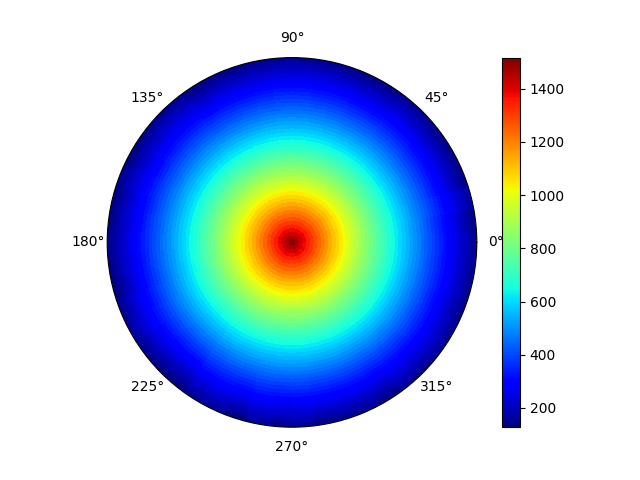
\includegraphics[width=\textwidth]{test.0}
\caption{Temperatura dentro del horno}
\label{fig:temperature}
\end{figure}

%\subsection{Matriz en "banda"}
%%TODO

\section{Gauss vs LU}

\paragraph{} Para resolver un sistema de ecuaciones cualquiera planteado como \(Ax = b\), se puede usar el método de eliminación gausseana (o "Gauss"), que tiene un tiempo de operación \(\bigO{n^3}\). Pero también se puede resolver usando la factorización \(LU\), que son dos matrices tales que \(A = LU\), y \(L\) es triangular inferior y \(U\) triangular superior. La forma de resolverlo así sería primero calcular un \(y\) tal que \(Ly = b\) y luego resolver \(Ux = y\). Esto toma \(\bigO{n^2}\) operaciones.
\paragraph{} Como vimos en la sección \ref{sec:justificacion}, la matriz de nuestro sistema tiene factorización \(M = LU\). Lo cual nos es muy útil cuando queremos resolver múltiples instancias de \(Mt_i = b_i\) ya que la factorización \(LU\) se puede calcular aplicando Gauss una sola vez, y resolver cada instancia \(LUt_i = b_i\) requiere muchas menos operaciones. \\
En la figura \ref{fig:solve.time} se puede ver que una vez que la matriz tiene 30 o más elementos, se vuelve definitivamente mejor resolver una instancia con \(LU\) que con Gauss. 

\begin{figure}[H]
\centering
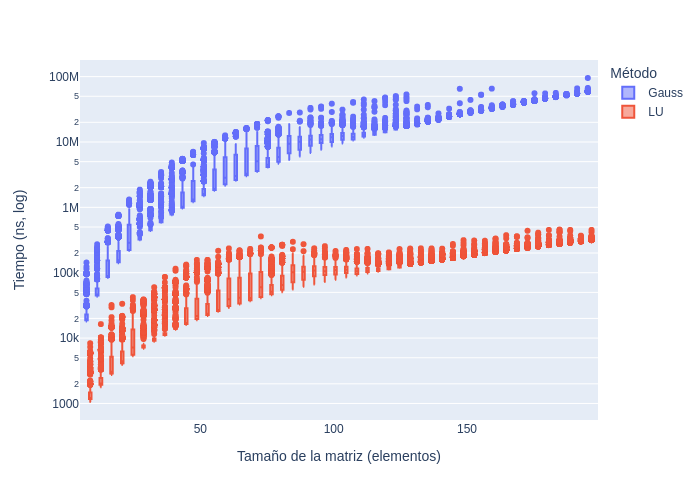
\includegraphics[width=\textwidth]{times.solve.1000.1}
\caption{Tiempo para resolver una instancia del sistema (1000 reps)}
\label{fig:solve.time.1000.1}
\end{figure}

\begin{figure}[H]
\centering
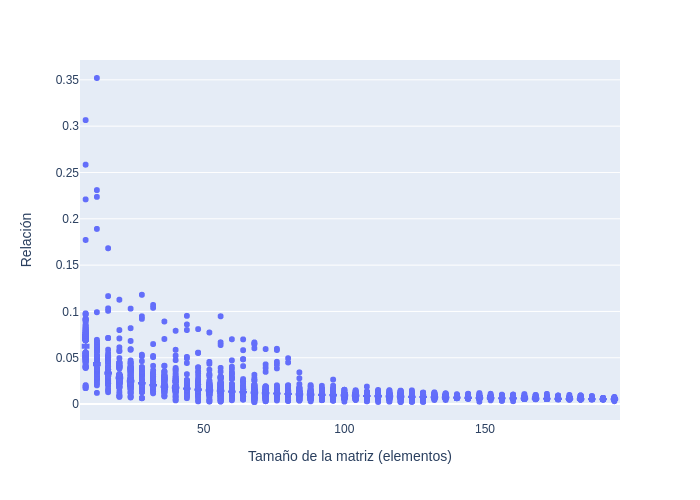
\includegraphics[width=\textwidth]{times.ratio_lu_gauss.1000.1}
\caption{Relación del tiempo entre LU y Gauss (1000 reps)}
\label{fig:solve.time.ratio}
\end{figure}


\paragraph{} Pero como mencionamos, para calcular la factorización hay que aplicar Gauss una vez, por lo que en realidad nos queda el resultado de la figura \ref{fig:solve.lu.time} para resolver una instancia. \\
Por lo que es importante revisar cuándo de verdad nos empieza a convenir usar la factorización \(LU\). En la figura \ref{fig:pct_lu.time} se ve que independiente del tamaño de la matriz, el tiempo usado para resolver una instancia del sistema es una fracción mínima del tiempo usado para calcular la factorización. Por lo que para dos o más instancias del sistema combiene calcular y usar la factorización \(LU\) (resaltado en la figura \ref{fig:time.2solve}).

%TODO: Gráfico mostrando lu+2solve vs 2Gauss

%\begin{figure}[H]
%\centering
%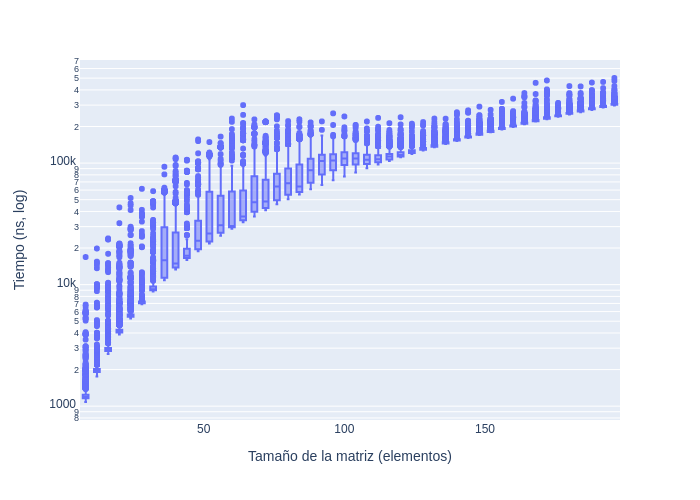
\includegraphics[width=\textwidth]{times.lu}
%\caption{Tiempo para calcular la factorización LU (1000 reps)}
%\label{fig:lu.time}
%\end{figure}

\begin{figure}[H]
\centering
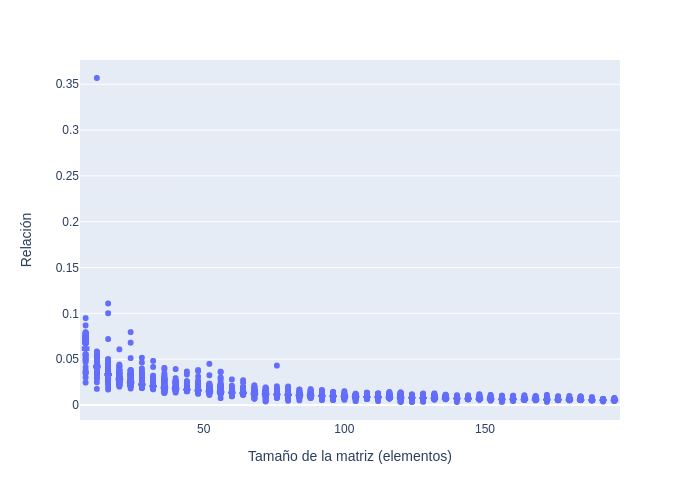
\includegraphics[width=\textwidth]{times.pct_lu.1000.1}
\caption{Relación entre el tiempo para resolver el sistema y el tiempo para calcular la factorización LU (1000 reps)}
\label{fig:pct_lu.time}
\end{figure}

\section{Estimando la isoterma}

\paragraph{} Un dato importante que nos interesa es encontrar la posición de la isoterma de 500ºC. Esta es un círculo dentro de la pared del horno todo a la misma temperatura. \\
Queremos poder calcularla porque si está "muy cerca" (ver sección \ref{sec:peligrosidad.distance}) la estructura del horno estaría en riesgo. %TODO: Hyperlink

\begin{figure}[H]
\centering
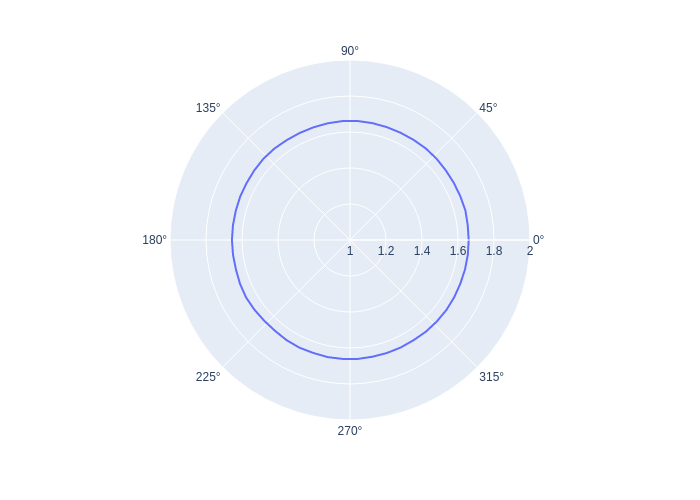
\includegraphics[width=\textwidth]{test.isotherm.0}
\caption{Posición de la isoterma}
\label{fig:isotherm.pos}
\end{figure}

\paragraph{} Para encontarla buscamos dos puntos dentro de un mísmo ángulo que "rodeen" la temperatura buscada, y luego aproximamos linealmente la posición donde se encuentra entre estos dos puntos.

%TODO: Diagrama mostrando la isoterma estimada entre dos puntos

\subsection{Midiendo la Peligrosidad}
\label{sec:peligrosidad.distance}

\paragraph{} Una vez encontrada la isoterma, es importante decidir si el horno está en un estado peligroso o seguro. Sabemos que si el exterior del horno llega a tener una temperatura de 500ºC o más, se rompe. \\
En la figura \ref{fig:peligrosidad.distance} se puede ver cómo se mueve la isoterma de 500ºC si la temperatura interna creciera uniformemente. \\

\begin{figure}[H]
\caption{Distancia de la isoterma al exterior del horno}
\centering
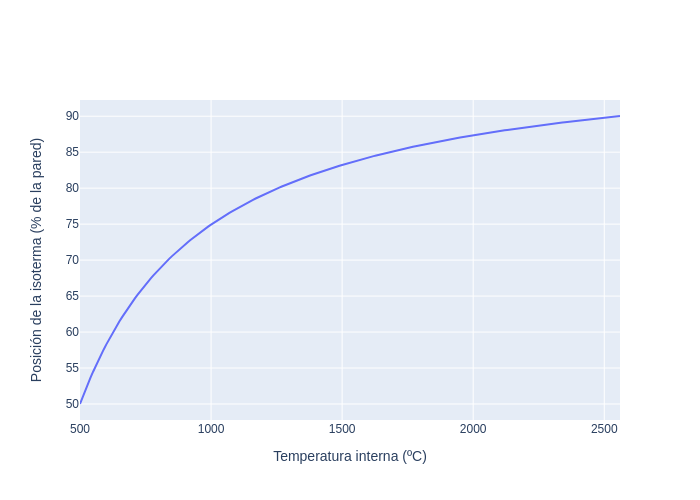
\includegraphics[width=\textwidth]{peligrosidad.distance}
\label{fig:peligrosidad.distance}
\end{figure}

\paragraph{} Para sacar conclusiones sobre qué tan peligroso es, habría que conocer más sobre los materiales que forman al horno. Pero preliminarmente se puede ver que si el "punto de ruptura" se encuentra al 75\% hay poco margen de error, ya que la isoterma se mueve rápido hacia el exterior.


\section{Demostración}

\section{Introducción teórica}


\textbf{\textit{En esta sección se presentan los elementos teóricos que soportan la resolución del trabajo práctico.}} 
\\

En el trabajo se estudia diferentes maneras de encontrar una isoterma en la pared de un alto horno. Para ello se necesitan las dimensiones del horno, como la cantidad de radios, ángulos y las temperaturas en las secciones exteriores e interiores del mismo. Para estudiar el calor en el interior del horno se debe discretizar los datos de temperatura, ya que no pueden ser evaluados de forma continua. 

Para plantear el problema es necesario armar un sistema de ecuaciones $Ax =b$ donde A sea una matriz de coeficientes obtenidos desde la ecuación de Laplace en la sección \ref{sec:EJEMPLO}, a partir de esa ecuación queda determinada la matriz tal como se explica en la sección \ref{sec:EJEMPLO_FUNCION_PARTIDA}. \\
Para resolver el sistema se realizan operaciones entre filas y columnas de la matriz $A$ y el vector $b$, es decir, se utiliza el algoritmo de eliminación 
Gausseana para obtener un sistema de ecuaciones que sea equivalente al sistema original, con el objetivo de simplificar las cuentas del mismo. Para ello, primero es necesario demostrar que la matriz $A$ cumple con la propiedad de ser \textbf{estrictamente diagonal dominante}, esto permite que las operaciones que se realicen nunca se vaya a realizar una permutación entre filas o columnas. 


\begin{defi}
	Sea ${A} \in \mathbb{R}^{n \times n}$. ${A}$ se dice \emph{diagonal dominante} si 
	\[
	\sum_{j = 1, j \neq i }^{n}|A_{ij}| \leq  |A_{ii}| \qquad \text{para todo $i = 1, \dots, n$}
	\]
	
\end{defi}

\begin{lema}
	\label{lema:{EG conserva diagonal dominante}
		Sea ${A}^{(0)} = {A} \in \mathbb{R}^{n \times n}$ una matriz diagonal dominante, con ${A}_{1,1} \neq 0$, y ${A}^{(1)}$ el resultado de aplicar un paso de Eliminación Gaussiana (sin pivoteo) sobre ${A}$. Entonces ${A}^{(1)}$ es diagonal dominante.
	\end{lema}
	\begin{proof}
		Consideremos la $k$-ésima fila de ${A}^{(1)}$, queremos ver que 
		$\lvert  a^{(1)}_{i,i} \rvert \geq \sum_{k = 1 \\ k \neq i}^n \lvert a^{(1)}_{i,k} \rvert$
		Se tiene que
		\[ \lvert a^{(1)}_{k,k} \rvert = \lvert a_{k,k} - \frac{a_{k,1}}{a_{1,1}} a_{1,k} \rvert
		\qquad \text{y} \qquad
		\sum_{\substack{i = 1 \\ i \neq j}}^n \lvert a^{(1)}_{j,i} \rvert
		= \sum_{\substack{i = 2 \\ i \neq j}}^n \lvert a_{j,i} - \frac{a_{j,1}}{a_{1,1}} a_{1,i} \rvert \]
		
		Ahora veamos como es un paso de eliminación gausseana:
		
		\[ \begin{split}
			\sum_{\substack{k = 1 \\ k \neq i}}^n \lvert a^{(1)}_{i,k} \rvert
			&= \sum_{\substack{k = 2 \\ k \neq i}}^n \lvert a_{i,k} - \frac{a_{i,1}}{a_{1,1}} a_{1,k} \rvert \\
			&\leq \sum_{\substack{k = 2 \\ k \neq i}}^n \vert a_{i,k} \vert + \left \vert \frac{a_{i,1}}{a_{1,1}} \right \vert \sum_{\substack{k = 2 \\ k \neq i}}^n \vert a_{1,i} \vert \\
			&\leq \left( \vert a_{i,i} \vert - \vert a_{i,1} \vert \right) + \left \vert \frac{a_{i,1}}{a_{1,1}} \right \vert \left( \vert a_{1,1} \vert - \vert a_{1,i} \vert \right) \\
			&= \vert a_{i,i} \vert - \left \vert \frac{a_{i,1}}{a_{1,1}} \right \vert \vert a_{1,i} \vert \\
			&\leq \left \vert a_{i,i} -  \frac{a_{i,1}}{a_{1,1}} a_{1,i} \right \vert = \lvert a^{(1)}_{i,i} \rvert 
		\end{split} \]
	\end{proof}
	
	Ahora se tiene que luego de realizar un paso de eliminación gausseana la matriz resultante también es diagonal dominante.
	
	Finalmente, queda demostrar, que luego de realizar una iteración del algoritmo de eliminación gaussiana sin pivoteo la matriz resultante queda bien definida.
	
	
	Entonces:
	\[ \begin{split}
		\lvert a_{i,i} \rvert &= \beta  = \left \vert - \frac{2}{(\Delta r)^2} + \frac{1}{r \Delta r} - \frac{2}{r^2 (\Delta \theta)^2} \right \vert \\
		&= \left \vert - \frac{1}{(\Delta r)^2} + \frac{1}{r \Delta r} - \frac{2}{r^2 (\Delta \theta)^2} - \frac{1}{(\Delta r)^2} \right \vert \\
		&= \left \vert - \frac{r - \Delta r}{r (\Delta r)^2} - \frac{2}{r^2 (\Delta \theta)^2} - \frac{1}{(\Delta r)^2} \right \vert \\
		&= \left \vert \frac{r - \Delta r}{r (\Delta r)^2} + \frac{2}{r^2 (\Delta \theta)^2} + \frac{1}{(\Delta r)^2} \right \vert
	\end{split} \]
	
	Veamos que si $r_{int}, \Delta r > 0$ y $j \geq 1$, se cumple que
	\[ r - \Delta r = (r_{int} + j \Delta r) - \Delta r = r_{int} + (j - 1) \Delta r > 0\]
	$\text{Entonces ahora sabemos que:}$
	\[ r - \Delta r > 0\]
	Ahora veamos como queda la sumatoria de las columnas. Notar que:	
	\[ \lvert a_{i,i} \rvert = \frac{r - \Delta r}{r (\Delta r)^2} + \frac{2}{r^2 (\Delta \theta)^2} + \frac{1}{(\Delta r)^2} \]
	
	Ahora al sumar los módulos del resto de los coeficientes, notar que en una fila pueden aparecer hasta 5 coeficientes por eso se suman el modulo de todos, asi queda que:
	\[ \begin{split}
		\sum_{\substack{k=1 \\ k \neq i}}^{(m-1)n} \vert a^{j}_{i,k} \vert &= \left \vert \frac{1}{(\Delta r)^2} - \frac{1}{r \Delta r} \right \vert + 2 \left \vert \frac{1}{r^2 (\Delta \theta)^2} \right \vert + \left \vert \frac{1}{(\Delta r)^2} \right \vert \\
		&= \left \vert \frac{r - \Delta r}{r (\Delta r)^2} \right \vert + \frac{2}{r^2 (\Delta \theta)^2} + \frac{1}{(\Delta r)^2} \\
		\text{y ahora por lo probado antes} \\
		&= \frac{r - \Delta r}{r (\Delta r)^2} + \frac{2}{r^2 (\Delta \theta)^2} + \frac{1}{(\Delta r)^2} = \rvert a_{i,i} \lvert
	\end{split} \]
	
	Asi de la demostración anterior se obtuvo que la matriz A es diagonal dominante y aparte no tieene 0 en la diagonal. Ahora resta ver que la eliminacion gausseana es aplicable y se puede utilizar sin pivoteo. Asi solamente hay que ver que para los puntos del medio del horno puede aplicarse eliminacion gausseana y ademas la matriz resultante es diagonal dominante. 
	
	\begin{itemize}
		\item Caso base: Notemos que $a_{1,1} = \beta$ no es nulo, ya que es un coeficiente definido mediante la ecuación de calor, entonces se puede aplicar el primer paso de Eliminación Gaussiana. Dado que $a_{1,2} = \chi$ pero como mostramos anteriormente $\beta \ge \chi$ entonces en el lugar $a_{2,2}$ queda un coeficiente no nulo y ya que la matriz luego de haber procesado la primer fila sigue siendo diagonal dominante entonces puedo aplicar el siguiente paso de eliminación gausseana.
		
		\item Caso inductivo: 
		\subitem 	Tomamos la hipótesis inductiva \textbf{(HI)}: la matriz ${A}^{(k-1)}$, obtenida tras aplicar $k-1$ pasos de eliminación gaussiana sobre ${A}$, es diagonal dominante y su k-ésima fila es no nula. Esto implica que $a^{(k-1)}_{k,k} \neq 0$.
		
		Vamos a escribir a $A^{(k-1)}$ por bloques de la siguiente manera:
		\[ {A}^{(k-1)} = \left( \begin{matrix} \bar{A}_{k-1} & {B} \\ {C} & \widetilde{{A}}_{k-1} \end{matrix} \right) \]
		luego de haber probado lo anterior, $\bar{A}_{k-1}$ y $\widetilde{{A}}_{k-1}$ son matrices diagonal dominantes.
		Dado la construcción del sistema la matriz $C$ no le queda otra que ser la matriz nula, ya que no hay coeficientes de la ecuación de calor para modificar los valores de esa matriz en ningun paso de Gauss.
		
		Entonces cuando se quiere aplicar un paso de eliminación gaussiana sobre $\widetilde{A}$, dado que el elemento de la diagonal es no nulo, este paso se puede hacer sin pivotear la matriz, y utilizando el lema \ref{lema:EG conserva diagonal dominante} se sigue que la matriz luego de este paso sera diagonal dominante.
		
		Solo resta probar que la fila $k+1$ de la matriz ${A}^{(k)}$ es no nula ya que si es nula entonces no se puede expresar el siguiente paso de la eliminación gausseana.
		
		Si la fila representa a un coeficiente de la ecuación de calor, para ciertos $j = 1, \dots, m - 1$ y $k = 0, \dots, n - 1$. Puntualmente, por la forma en la que se construye la matriz del sistema, el elemento $a_{k+1,k+1+m o n nose}$ es el coeficiente de la temperatura $t_{j,k+1}$ en dicha ecuación, debe ser no nulo. Dado como esta armado el sistema todos los elementos de la columna $k+1$ que se encuentran por arriba de $a_{k+1,k+1+m o n nose}$, deben ser nulos, es decir, en una iteracion de gauss no deberían haberse modificado el coeficiente $a_{k+1,k+1+m o n nose}$ entonces sigue siendo no nulo.
	\end{itemize}
	




\section{Apéndice}

\tableofcontents

\listoffigures

\end{document}

%TODO: Math formatting
